\documentclass[12pt]{article}
\bibliographystyle{plain}

\usepackage{hyperref}
\usepackage[sc]{mathpazo}
\usepackage[utf8]{inputenc}
\usepackage{graphicx}
\usepackage{subfigure}
\title
{
Advanced Methods Tutorial
}

\author{Kyle Beauchamp \and TJ Lane \and Greg Bowman \and  Robert McGibbon \and Vijay Pande}

\begin{document}

\maketitle

\section{Table of Contents}
\begin{enumerate}
\item Ward Clustering
\item SCRE Rate matrix estimation
\end{enumerate}

\newpage

\subsection{Cluster your data using Ward's algorithm and the RMSD metric}

MSMBuilder provides multiple clustering algorithms.  In the 'basic' tutorial, we used a hybrid k-centers k-medoids algorithm.  That algorithm is quite fast, but more advanced clustering algorithms can lead to better models.  In particular, we have found that
Ward clustering provides two key advantages over k-centers \cite{beauchamp2012simple}:

\begin{enumerate}
 \item Improved statistics in each state--that is, few states will have ``poor'' statistics.
 \item Ward clustering typically leads to slower, more converged implied timescales.  This is due Ward better separating kinetically distinct regions of conformation space.
\end{enumerate}

Note that the key disadvantage of Ward is that it requires large amounts of memory.  


WARNING: this step requires a minimum of 3.0 GB of memory for storing a matrix of pairwise RMSD.
\begin{verbatim}
Cluster.py rmsd hierarchical
\end{verbatim}

As example, the following figure shows that Ward clustering leads to improved implied timescales, as compared to Hybrid clustering:

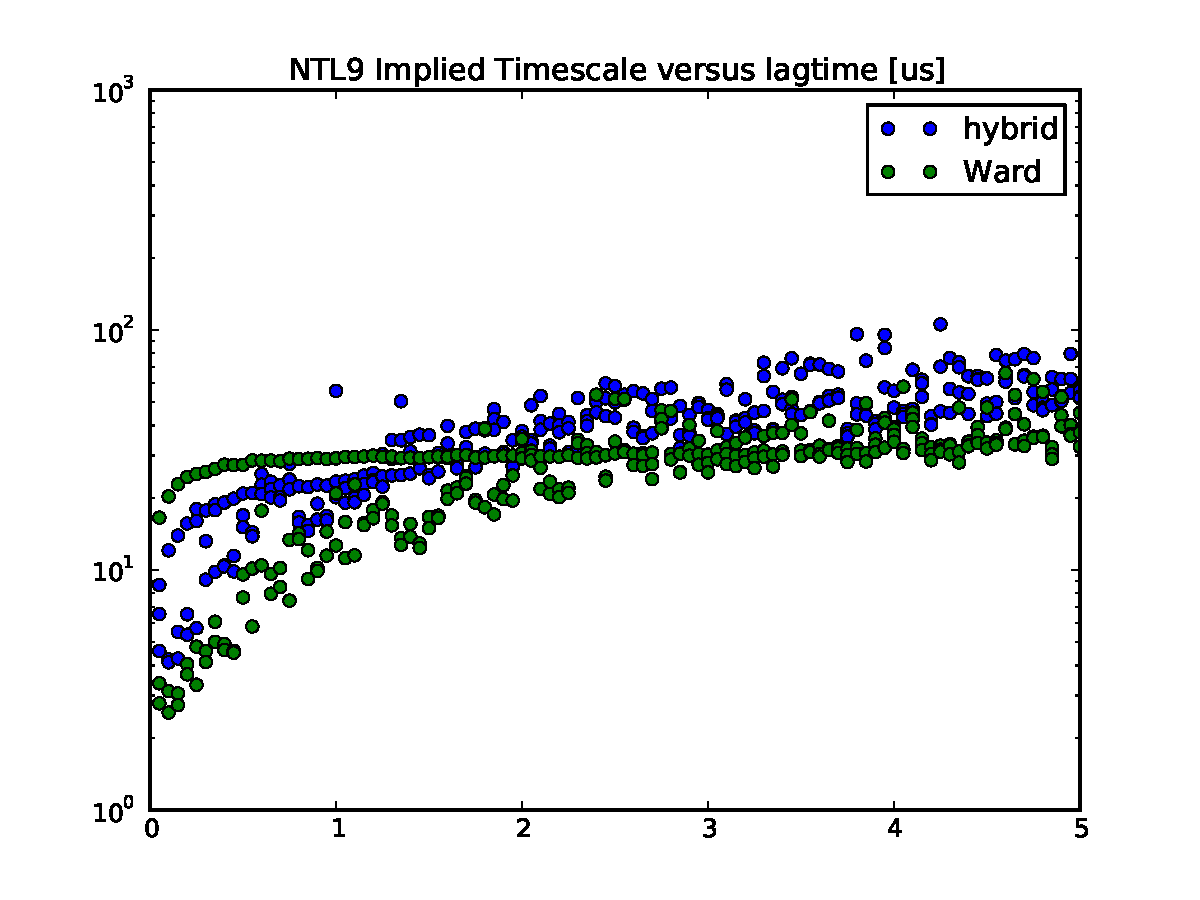
\includegraphics[width=11.7cm]{figures/NTL9-Timescales.pdf}


\subsubsection{Estimate a rate matrix using SCRE}

In the macrostate implied timescales, the slowest implied timescale converges at approximately 10 ps, while the third timescale converges as 5 ps.  Furthermore, the third timescale is aliased at lagtimes starting with 14 ps; lagtimes longer than 14 ps will not accurately capture the dynamics of this relaxation.  This suggests that this system might benefit from estimating rates using SCRE and multiple lagtimes \cite{beauchamp2012simple}.  Note that SCRE currently is practical only for models with few states ($n \le 10$).  

To build an SCRE model, we first construct a macrostate transition matrix with lagtime 1.  

\begin{verbatim}
 BuildMSM.py -l 1 -a Macro4/MacroAssignments.h5 -o Macro4/
\end{verbatim}

The key idea in SCRE is to estimate rate matrix $K_{ij}(\tau)$ for a variety of lagtimes.  Then, each rate matrix element is fixed when $K_{ij}(\tau)$ becomes approximately constant with respect to the lagtime $\tau$.  The final rate matrix provides estimates of Markovian rates for each of the rate elements $K_{ij}$.  

Next, we run an interactive script to estimate rates using SCRE.  

\begin{verbatim}
 Interactive-SCRE.py -a Macro4/Assignments.Fixed.h5 -o Macro4
\end{verbatim}

In practice, the script will prompt the user to select a maximum lagtime.  The script then estimates and plots rate matrices for each lagtime up to the maximum value.  The user is then asked to identify converged rate matrix elements.  In general, one should try to estimate the quickly-convergign rates first.  After those rates are constrained, one can then try to estimate the slower and / or less Markovian rates.  For concreteness, I used the following inputs:

25
1,0,6
25
3,2,19
25
3,1,6
25
3,0,9
25
14

Note that on the last iteration, the user is asked only to select a lagtime.  Also note that your choices may be different because of differences in the macrostate definitions; the PCCA+ minimization uses a non-deterministic simulated annealing.  Also, if your state decomposition is insufficiently Markovian, you may find that the plotted rate estimates show a ``periodic'' behavior.  This likely indicates that a given macrostate contains multiple slowly interconverting substates; as you increase the lagtime, the model switches from the faster process to the slower process.  In such situations, your best bet is to increase the number of macrostates.  

Finally, we compare the fixed-lagtime and SCRE estimates of implied timescales:

\begin{verbatim}
 python PlotMacrostateImpliedTimescales.py
\end{verbatim}


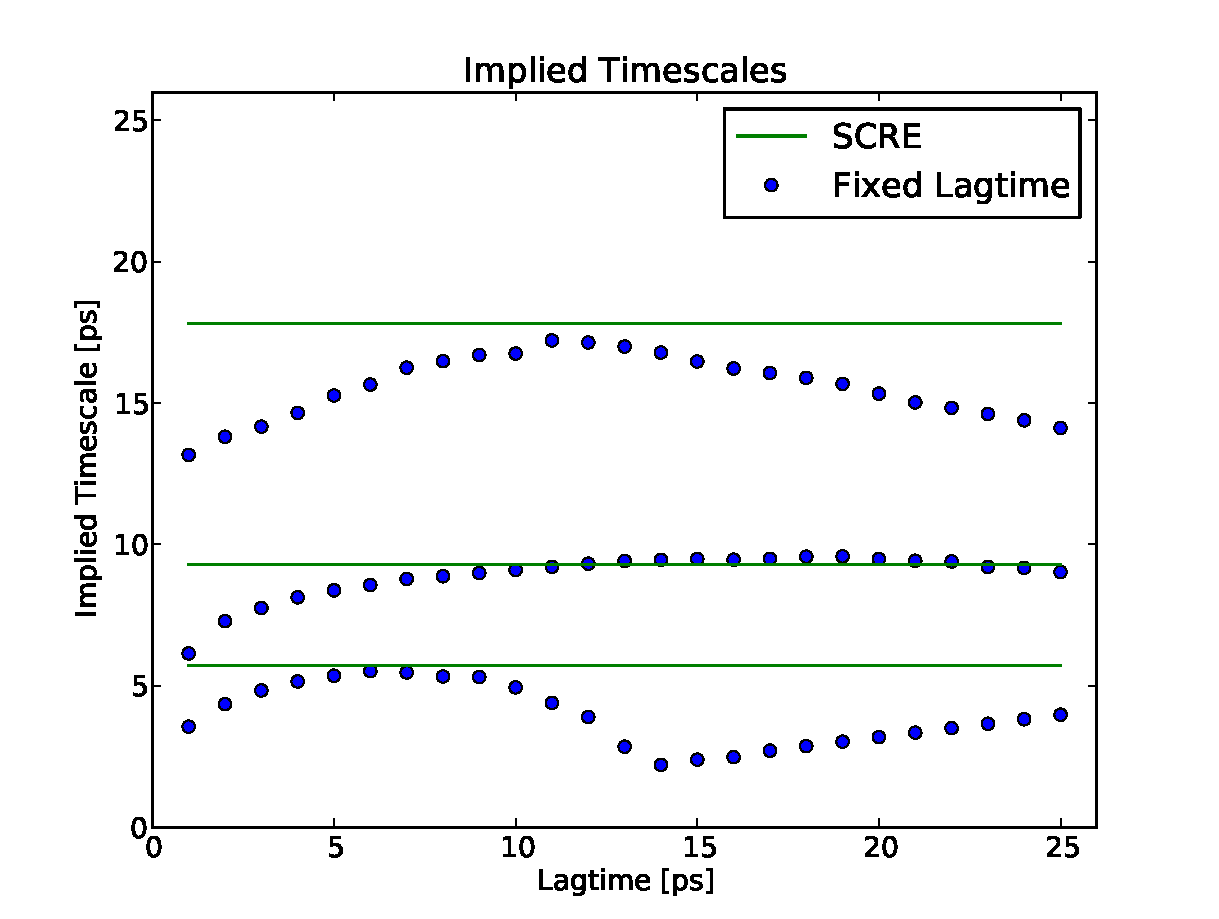
\includegraphics[width=11.7cm]{figures/SCRE}


We find that the SCRE estimates capture the ``converged'' values of the fixed-lagtime timescales.  Achieving convergence for each timescale is not possible with a fixed-lagtime MSM, because the 20 ps lagtime required for the second relaxation causes the third relaxation to alias.  

\newpage



\bibliography{AdvancedMethods}


\end{document}